\pagebreak
W przypadku kroswalidacji stratyfikowanej wyniki się tylko niezmiernie różnią. Można
zauważyć bardzo podobne wzorce w wartościach miar (CAIM wypada bardzo słabo). Inną różnicą
jest parametr kroswalidacji, dla którego miara F1 osiąga najwyższą wartość -- tym razem
jest to $K = 6$.
\begin{figure}[H]
\center
    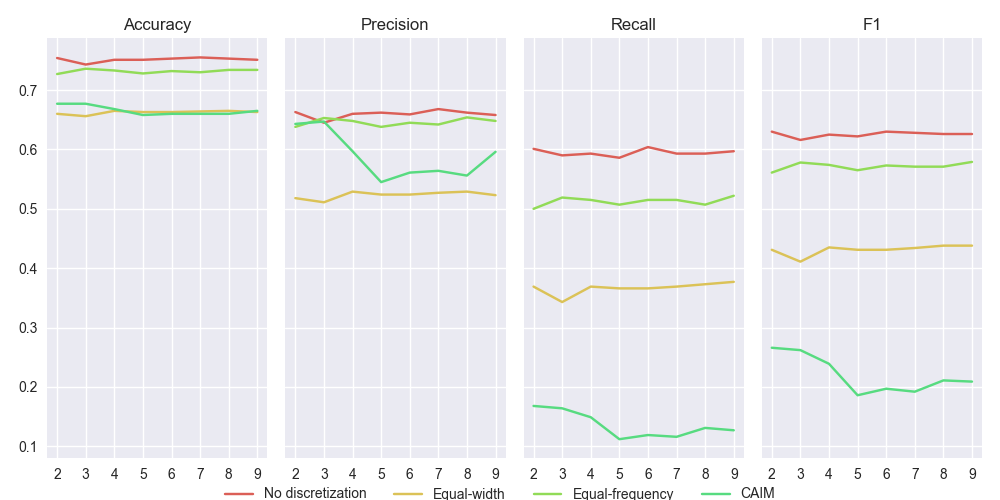
\includegraphics[width=\textwidth]{img/cv_scores_stratifiedkfold/scoring_stratifiedkfold_diabetes.png}
    \caption{Wykresy wartości metryk dla zbioru "Diabetes" -- kroswalidacja stratyfikowana.}
\end{figure}

Podobnie macierz konfuzji również jest prawie identyczna jak w przypadku kroswalidacji zwykłej.
Różnica jest na poziomie 0.01 dla zdrowych osób. Wniosek jest tutaj taki, że skoro stratyfikacja
nie pomogła, to rozkład instancji w zbiorze danych jest w miarę zbalansowany i nawet przy podziale
na podzbiory nie zostaje mocno zaburzony.

\begin{figure}[H]
\center
    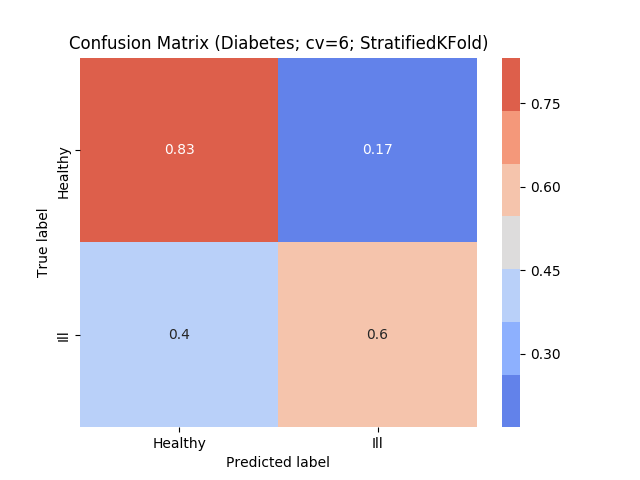
\includegraphics[width=0.6\textwidth]{img/conf_matrices/cm_Diabetes_cv6_StratifiedKFold.png}
    \caption{Macierz konfuzji dla najlepszej wartości F1 -- kroswalidacja stratyfikowana.}
\end{figure}

\begin{table}[H]
\center
    \caption{Wartości metryk dla zbioru "Diabetes" -- kroswalidacja stratyfikowana.}
    \begin{tabular}{|c|c|c|c|c|c|c|c|c|c|}
        \hline
        \multirow{2}{*}{\textbf{Metoda dyskr.}} & \multirow{2}{*}{\textbf{Metryka}} & \multicolumn{8}{|c|}{\textbf{CV}} \\ \cline{3-10}
                        &  & 2 & 3 & 4 & 5 & 6 & 7 & 8 & 9 \\ \hline
        \multirow{4}{*}{\textit{Brak}}  & Accuracy & 0.754 & 0.743 & 0.751 & 0.751 & 0.753 & 0.755 & 0.753 & 0.751 \\ \cline{2-10}
                                         & Precision & 0.663 & 0.645 & 0.66 & 0.662 & 0.659 & 0.668 & 0.662 & 0.658 \\ \cline{2-10}
                                         & Recall & 0.601 & 0.59 & 0.593 & 0.586 & 0.604 & 0.593 & 0.593 & 0.597 \\ \cline{2-10}
                                         & F1 & 0.63 & 0.616 & 0.625 & 0.622 & 0.63 & 0.628 & 0.626 & 0.626 \\ \hline \hline


        \multirow{4}{*}{\textit{Equal-width}}  & Accuracy & 0.66 & 0.656 & 0.665 & 0.663 & 0.663 & 0.664 & 0.665 & 0.663 \\ \cline{2-10}
                                             & Precision & 0.518 & 0.511 & 0.529 & 0.524 & 0.524 & 0.527 & 0.529 & 0.523 \\ \cline{2-10}
                                             & Recall & 0.369 & 0.343 & 0.369 & 0.366 & 0.366 & 0.369 & 0.373 & 0.377 \\ \cline{2-10}
                                             & F1 & 0.431 & 0.411 & 0.435 & 0.431 & 0.431 & 0.434 & 0.438 & 0.438 \\ \hline \hline


        \multirow{4}{*}{\textit{Equal-freq}}  & Accuracy & 0.727 & 0.736 & 0.733 & 0.728 & 0.732 & 0.73 & 0.734 & 0.734 \\ \cline{2-10}
                                             & Precision & 0.638 & 0.653 & 0.648 & 0.638 & 0.645 & 0.642 & 0.654 & 0.648 \\ \cline{2-10}
                                             & Recall & 0.5 & 0.519 & 0.515 & 0.507 & 0.515 & 0.515 & 0.507 & 0.522 \\ \cline{2-10}
                                             & F1 & 0.561 & 0.578 & 0.574 & 0.565 & 0.573 & 0.571 & 0.571 & 0.579 \\ \hline \hline


        \multirow{4}{*}{\textit{CAIM}}  & Accuracy & 0.677 & 0.677 & 0.668 & 0.658 & 0.66 & 0.66 & 0.66 & 0.665 \\ \cline{2-10}
                                         & Precision & 0.643 & 0.647 & 0.597 & 0.545 & 0.561 & 0.564 & 0.556 & 0.596 \\ \cline{2-10}
                                         & Recall & 0.168 & 0.164 & 0.149 & 0.112 & 0.119 & 0.116 & 0.131 & 0.127 \\ \cline{2-10}
                                         & F1 & 0.266 & 0.262 & 0.239 & 0.186 & 0.197 & 0.192 & 0.211 & 0.209 \\ \hline \hline

            \hline
    \end{tabular}
\end{table}

